%% =====================================================================
%% elsarticle-IJEC.tex
%% English manuscript formatted with Elsevier's elsarticle document class
%% (numbered reference style) for AEU - International Journal of
%% Electronics and Communications.
%% Translated and adapted from articuloCompleto.tex (IEEEtran, Spanish).
%% Compile with:  pdflatex -> bibtex -> pdflatex -> pdflatex
%% =====================================================================
%% 'review' gives the double-spaced single-column 12pt layout required by the
%% journal's review formatting. AEU/IJEC uses the numbered (Vancouver) citation
%% style, so 'authoryear' is intentionally omitted and elsarticle-num is used.
%% For a final journal layout use, e.g., [final,1p,times].
\documentclass[preprint,review,12pt]{elsarticle}

\usepackage{amssymb}
\usepackage{amsmath}
\usepackage{graphicx}
\usepackage{multirow}
\usepackage{textcomp}
%% AEU/IJEC review formatting: 12pt, single column, double-spaced (from the
%% 'review' class option) and 1-inch margins (enforced here).
\usepackage[margin=1in]{geometry}
\usepackage[hidelinks]{hyperref}
\usepackage{orcidlink}

\journal{AE\"U -- International Journal of Electronics and Communications}

\begin{document}

\begin{frontmatter}

\title{Equalization Co-Design for Maximizing Viable Symbol Rate in Bandwidth-Limited High-Speed Interconnect Links}

\author[inst1]{Segundo Francisco Segura-Altamirano\corref{cor1}\,\orcidlink{0000-0002-0103-7222}}
\ead{sseguraal@unprg.edu.pe}

\author[inst1]{Diana Mercedes Castro-C\'ardenas\,\orcidlink{0000-0001-8489-9671}}
\ead{dcastroc@unprg.edu.pe}

\affiliation[inst1]{organization={Universidad Nacional Pedro Ruiz Gallo},
            city={Lambayeque},
            country={Peru}}

\cortext[cor1]{Corresponding author.}

\begin{abstract}
Copper interconnects on printed circuit boards and silicon behave, in the
bandwidth-limited regime, as channels whose loss grows with frequency, so
intersymbol interference closes the eye diagram as the signaling rate
rises. The distributed RC model used in these studies idealizes the
channel by omitting frequency-dependent skin-effect and dielectric losses,
and studies often overestimate the bit error rate by injecting noise after
the equalizer gain. This work quantifies how much viable symbol rate each
equalization stage contributes, first on a distributed RC channel
validated against its analytical transfer function and then on dispersive
physical channels representing board substrates of differing loss. The
transmit feed-forward and receive linear equalizers are co-designed by
Latin hypercube sampling; the receiver includes input-referred noise and
finite bandwidth; and results are verified against an independent circuit
simulator. On the RC channel, the viable rate grows from 2.9 to 9.8~GBaud
with the co-designed equalizers, reaching 13.7~GBaud with a
decision-feedback equalizer. At equal loss, dispersive channels tolerate a
higher unequalized rate, and the co-design must be re-optimized per
substrate. Jointly co-optimizing linear boost and decision feedback
outperforms stage-by-stage tuning, the timing margin stays robust, and an
eight-level stress case confirms the method generalizes.
\end{abstract}

\begin{highlights}
\item Viable symbol rate quantifies the gain of each equalization stage per channel
\item RC idealization overstates link difficulty versus dispersive lines at equal loss
\item Equalizer co-design must be re-optimized per substrate on the physical channel
\item Joint co-optimization of linear boost and decision feedback beats staged tuning
\item Input-referred noise prevents overestimating the equalizer benefit and the BER
\end{highlights}

\begin{keyword}
distributed RC interconnect \sep signal integrity \sep channel
equalization \sep continuous-time linear equalizer \sep
decision-feedback equalizer \sep intersymbol interference \sep design of experiments
\end{keyword}

\end{frontmatter}

%% =====================================================================
\section{Introduction}
\label{sec:intro}

Copper interconnects on printed circuit boards and on silicon behave, in
the bandwidth-limited regime, as distributed-parameter channels whose
resistive and capacitive loss grows with frequency; as the signaling rate
increases, the channel bandwidth becomes insufficient and intersymbol
interference (ISI) closes the eye diagram \citep{10370948}. For these
interconnects, the distributed RC line model describes the response with
greater fidelity than a lumped RC model \citep{761200}, and its diffusive
behavior---delay and rise-time degradation that grow along the line---is
captured by ladder networks of $N$ cells \citep{5697500}.

The RC model, however, idealizes the channel. At frequencies of several
gigahertz, the loss of copper traces is frequency dependent, with a
conductor component associated with the skin effect and a dielectric
component that grows with frequency \citep{9888577,915226}. These
mechanisms, absent from the diffusive RC model, turn the channel into a
dispersive one, with propagation delay and attenuation governed by the
substrate; a transmission-line model with frequency-dependent distributed
parameters describes them and allows the resulting eye diagram to be
estimated \citep{8861405,7445206}. The magnitude of the loss varies across
substrates, for example between standard FR-4 and low-loss-tangent
laminates \citep{9785524,10385078}.

Modern serial links mitigate ISI by combining a transmit feed-forward
equalizer (FFE), a receive continuous-time linear equalizer (CTLE) and a
decision-feedback equalizer (DFE) \citep{10260232,10811094}. Because these
stages interact and their tuning depends on the channel, their parameters
are usually co-designed rather than tuned in isolation \citep{11169790}.

Four-level pulse-amplitude modulation (PAM-4) has become the reference
multilevel scheme for bandwidth-limited channels, since it transmits two
bits per symbol at half the symbol rate and thus relaxes the bandwidth
requirement relative to NRZ signaling \citep{7964959,7193371}. Higher
orders, such as PAM-8, increase the bits per symbol at the cost of a
smaller noise margin and have been explored in bandwidth-limited systems
\citep{8963973}.

Two limitations recur in exploratory studies. First, bit error rate (BER)
evaluation: measuring a low BER by Monte Carlo counting requires
simulating a prohibitive number of bits in computation and memory
\citep{6248821}, so semi-analytical and statistical-eye methods are used
that reproduce the result at a much lower cost \citep{7202856,10415105}.
Second, receiver rigor: if noise is injected after the equalizer gain, the
signal-to-noise ratio is overestimated, since the equalizer boost also
amplifies out-of-band noise \citep{9707817}. In addition, the exploration
of the equalization space---whose number of combinations grows with the
rate---is addressed efficiently through design of experiments (DoE)
\citep{7851249}.

This work quantifies, first on a distributed RC channel validated against
its analytical transfer function, how much additional symbol rate each
equalization stage contributes, expressed as a reach metric. It then
extends the analysis to dispersive physical channels---FR-4 and
Megtron~6 substrates---and examines to what extent the co-design obtained
on the RC model transfers to the physical channel, re-optimizing it per
substrate where appropriate. The FFE+CTLE co-design is obtained by Latin
hypercube sampling, a DFE is added at the receiver, and quality is
assessed by the eye opening and a semi-analytical BER computed with
input-referred noise and finite bandwidth, so that the equalizer gains are
not overestimated. The joint co-optimization of the linear and feedback
stages and the link timing margin under random and deterministic jitter
are also examined. A PAM-8 stress case probes the generality of the
method. The contribution of this work does not lie in proposing a new
equalizer architecture or a new channel theory, but in quantifying, under
a single reproducible test bench and with input-referred receiver noise,
how much an equalization co-design optimized on an idealized RC channel
transfers---or does not---to physical dispersive channels. The remainder
of the article describes the channel model and methodology
(Section~\ref{sec:method}), reports the results
(Section~\ref{sec:results}), discusses them against the hypothesis
(Section~\ref{sec:discussion}) and concludes
(Section~\ref{sec:conclusion}).

%% =====================================================================
\section{Channel model and methodology}
\label{sec:method}

\subsection{Distributed RC channel model}
The channel is described as a distributed-parameter RC line. Neglecting
inductance and conductance, the telegrapher's equations reduce to the
diffusion equation
\begin{equation}
\frac{\partial^2 v(x,t)}{\partial x^2} = R_0 C_0\,\frac{\partial v(x,t)}{\partial t},
\label{eq:difusion}
\end{equation}
whose transfer function, for a line of length $d$ with an open-circuit
termination, is
\begin{equation}
H(s) = \frac{1}{\cosh\!\left(\sqrt{s\,R_t C_t}\right)},\qquad R_t=R_0 d,\ \ C_t=C_0 d.
\label{eq:cosh}
\end{equation}
Since \eqref{eq:cosh} is transcendental, it is approximated by a ladder
network of $N$ R--C cells represented in state space
($\dot{\mathbf{v}}=\mathbf{A}\mathbf{v}+\mathbf{B}u$,
$y=\mathbf{C}\mathbf{v}$) \citep{5152908,5697500}; alternatively, a
rational Pad\'e approximation may be used \citep{554593}. The validity of
the approximation is verified by comparing its Bode plot with that of
\eqref{eq:cosh} (Section~\ref{sec:results}). The reference channel has
$R_t=80\,\Omega$ and $C_t=5\,\mathrm{pF}$ ($R_tC_t=400\,\mathrm{ps}$,
$-3\,\mathrm{dB}$ bandwidth $\approx 0.95\,\mathrm{GHz}$); the time
constant scales as $R_tC_t\propto d^2$.

\subsection{Dispersive physical channel model}
To overcome the diffusive idealization, a transmission line with
frequency-dependent losses is additionally considered. The per-unit-length
parameters incorporate a series resistance with skin effect and a
dielectric conductance,
\begin{equation}
R(f)=\sqrt{R_{dc}^2+\left(k_s\sqrt{f}\right)^2},\qquad G(f)=2\pi f\,C\,\tan\delta,
\label{eq:rlgc}
\end{equation}
so that the propagation constant
$\gamma(f)=\sqrt{(R+j\omega L)(G+j\omega C)}=\alpha(f)+j\beta(f)$ exhibits
an attenuation that grows with frequency \citep{9888577,8861405}. The model
is parameterized for two representative substrates, FR-4
($\tan\delta\approx0.020$) and Megtron~6 ($\tan\delta\approx0.004$)
\citep{9785524,10385078}, and both are compared under two criteria: the
same insertion loss as the RC channel at the Nyquist frequency of the
nominal $4\,\mathrm{GBaud}$ operating point (that is, at $2\,\mathrm{GHz}$;
the \textit{equal\_il} criterion matches the loss at that frequency and
does not imply equal severity when the swept rate exceeds the nominal
point), and a common physical length of $10$~inches (the \textit{fixed}
criterion). The channel, in its RC or dispersive form, is applied in the
frequency domain through its transfer function; the equivalence with the
time-domain simulation is verified by reproducing, through the $N=5$
ladder, the reference result (Section~\ref{sec:results}) \citep{7445206}.
As an independent verification of the model and its implementation, the
scattering parameters of the channel are exported to Touchstone format and
the chain is additionally reproduced in a circuit simulator (LTspice),
contrasting both paths with the frequency-domain evaluation
(Section~\ref{sec:results}).

\subsection{Test source}
The link is excited with a pseudorandom binary sequence (PRBS) generated
by a linear-feedback shift register (PRBS23, primitive polynomial) with a
fixed seed, which guarantees the reproducibility of the experiment. The
sequence presents a balance close to $50\%$ and the worst-case
transitions that stress the channel ISI. The 30 independent realizations
used in the sweeps do not change the register seed: each realization takes
a \emph{disjoint window} of the same PRBS23 sequence and a \emph{paired
noise realization} (noise seed $1000{+}r$ for realization $r$, identical
across channels and configurations so that the comparison is paired and
fair). Thus, the reported variability comes from the data pattern and the
noise, not from a change of the generator seed.

\subsection{Modulation}
Gray-coded PAM-4 signaling is used, with equispaced levels in
$\pm 3\,\mathrm{V}$ and two bits per symbol, which halves the bandwidth
requirement relative to NRZ signaling \citep{7964959}. The demonstrator
operating point is $4\,\mathrm{GBaud}$ (Nyquist frequency $2\,\mathrm{GHz}$)
with oversampling of 32 samples per symbol. As a stress case, PAM-8 is
used (eight levels within the same $\pm 3\,\mathrm{V}$ amplitude budget,
with a level spacing $\approx 2.3\times$ smaller), representative of dense
constellations in bandwidth-limited systems \citep{8963973}.

\subsection{Equalizers and receiver}
The equalization chain combines three stages, as is common in high-speed
serial links \citep{10260232,10811094}. At the transmitter, a three-tap FIR
feed-forward equalizer (FFE)
\begin{equation}
x_{\mathrm{eq}}[n] = c_{-1}\,x[n{+}1] + c_{0}\,x[n] + c_{1}\,x[n{-}1],
\label{eq:ffe}
\end{equation}
with amplitude normalization (swing constraint) $\sum_i |c_i|=1$, which
bounds the excursion of the pre-emphasized signal and must not be confused
with a power constraint ($\sum_i c_i^2$). At the receiver, a one-zero,
two-pole continuous-time linear equalizer (CTLE) \citep{10873709}
\begin{equation}
H_{\mathrm{CTLE}}(s) = A_{DC}\,\frac{1+s/\omega_z}{(1+s/\omega_{p1})(1+s/\omega_{p2})},
\label{eq:ctle}
\end{equation}
with $A_{DC}=2.5$, $\omega_{p1}=2\pi\!\cdot\!15\,\mathrm{GHz}$ and
$\omega_{p2}=2\pi\!\cdot\!30\,\mathrm{GHz}$. Finally, a decision-feedback
equalizer (DFE) cancels the ISI post-cursors,
\begin{equation}
y_{\mathrm{eq}}[n] = y[n] - \sum_{i\ge 1} b_i\,\hat{x}[n{-}i],
\label{eq:dfe}
\end{equation}
whose coefficients are estimated by least squares from the transmitted
sequence and the aligned samples (data-aided fitting), which avoids the
phase mismatch between the design pulse and the sampling instant when the
channel exhibits propagation delay \citep{11346689}. Because it is
estimated with the known transmitted sequence, the decision feedback here
operates in an aided condition (a performance bound) and not as a blind
adaptive implementation; this condition bounds the interpretation of all
figures that include it. The receiver incorporates
\emph{input-referred AWGN} (injected at the channel output, before the
CTLE, with $\sigma_{in}=0.10\,\mathrm{V}$) and a \emph{finite-bandwidth
filter} ($\approx$ symbol rate). In this way the CTLE amplifies signal and
noise alike, and its benefit comes from the frequency boost, avoiding the
SNR overestimation that occurs when noise is injected after the equalizer
gain \citep{9707817}.

\subsection{Co-design by design of experiments}
Since the number of equalization combinations grows with the rate, the
co-design space is explored with design of experiments (DoE) rather than
exhaustive search \citep{7851249,5770781}. Latin hypercube sampling is
applied over the two variables that dominate the eye opening---the CTLE
zero $\omega_z$ and the FFE post-cursor $c_{post}$---with 30 samples; the
objective is the actual vertical opening of the worst eye ($3\sigma$
margin to ISI). The selected point is fixed for the subsequent
simulations. For the dispersive channels, since the optimal tuning depends
on the channel loss profile, the co-design is re-optimized per substrate
on the physical channel \citep{11169790}. The optimization can be performed
in stages---taking the linear-equalizer eye opening as the
objective---or jointly over the full chain---taking the viable rate with
decision feedback as the objective and incorporating the CTLE gain
$A_{DC}$ into the design space---to prevent an excessive linear boost from
penalizing the feedback stage. The framework admits extension to
sequential or Bayesian-optimization schemes \citep{11309336}.

\subsection{Evaluation variables and indicators}
The evaluation is structured on the operationalization of two variables.
The \emph{independent variable} is the co-designed equalization strategy,
whose dimensions are the TX-FFE, RX-CTLE and RX-DFE stages
(\eqref{eq:ffe}--\eqref{eq:dfe}) and the DoE tuning described above. The
\emph{dependent variable} is the link performance, measured by three
end-point indicators:

\begin{itemize}
\item \textbf{Rate reach} (primary indicator): viable symbol rate, defined
as the interpolated crossing---on a $\log_{10}(\mathrm{BER})$
scale---of the pre-FEC threshold ($\mathrm{BER}\le 10^{-2}$) in a rate
sweep; its value is reported as mean $\pm$ standard deviation over 30
independent PRBS-pattern and noise realizations. The $10^{-2}$ threshold
is compatible with a strong forward error correction (FEC) of the KP4/RS
family common in high-speed links; since it depends on the assumed FEC
scheme and is not universal, it is complemented by a sensitivity analysis
to stricter thresholds ($10^{-3}$ and $10^{-4}$,
Section~\ref{sec:results}).
\item \textbf{Signal integrity (vertical margin)}: worst-eye opening,
measured as the $3\sigma$ margin between adjacent PAM levels at the
optimal sampling instant.
\item \textbf{Timing margin (horizontal margin)}: horizontal eye opening,
obtained from the error-rate curve versus the sampling phase, injecting
random (Gaussian) and deterministic (dual-Dirac worst-case, or sinusoidal
periodic) jitter at the receiver sampling instant \citep{805809,9874925}.
The horizontal opening is obtained by equal-error-rate interpolation on
the bathtub curve, in line with BER-based eye reconstruction methods
\citep{Chen2024BER}.
\item \textbf{Reliability}: \emph{semi-analytical} BER; after aligning the
received signal with the transmitted symbols, the mean $\mu_k$ and the
standard deviation $\sigma_k$ of each level are estimated and the error
probability is extrapolated with the $Q(\cdot)$ function relative to the
decision thresholds, avoiding the prohibitive cost of Monte Carlo counting
of low BERs \citep{6248821,7202856,10415105}. This estimate assumes
Gaussian tails per level, an assumption that conditions the interpretation
of all BER and viable-rate results and that is contrasted against Monte
Carlo counting in the feasible region (Section~\ref{sec:results}).
Estimates below $10^{-12}$ are reported as \emph{below the reporting floor}
(extrapolated BER $<10^{-12}$), since in that region the Gaussian tail is
no longer reliable.
\end{itemize}

This procedure is consistent with the statistical-eye and peak-distortion
analysis approaches used to evaluate high-speed links with equalization
\citep{10705630}. Table~\ref{tab:params} summarizes the complete set of
test-bench parameters, so that the result tables are reproducible from a
single recipe.

%% Master table of simulation parameters (reproducibility).
\begin{table*}[!t]
\caption{Complete set of test-bench parameters (reproducibility).}
\label{tab:params}
\centering
\footnotesize
\begin{tabular}{p{0.20\textwidth} p{0.36\textwidth} p{0.36\textwidth}}
\hline
\textbf{Group} & \textbf{Parameter} & \textbf{Value} \\
\hline
\multirow{3}{*}{RC channel}
 & Total resistance/capacitance; time constant & $R_t=80\,\Omega$, $C_t=5\,\mathrm{pF}$, $\tau=R_tC_t=400\,\mathrm{ps}$ \\
 & Ladder approximation; $-3$~dB bandwidth & $N=5$ R--C cells (state space); $\approx0.97\,\mathrm{GHz}$ \\
 & Analytical reference transfer function & $H(s)=1/\cosh(\sqrt{s\,R_tC_t})$ \\
\hline
\multirow{5}{*}{Physical lines (RLGC)}
 & Microstrip geometry (common) & $Z_0=50\,\Omega$, width $w=150\,\mu\mathrm{m}$, thickness $t=35\,\mu\mathrm{m}$ (1~oz) \\
 & FR-4 / Megtron~6 substrate & $D_k=4.3$, $\tan\delta=0.020$ / $D_k=3.6$, $\tan\delta=0.004$ \\
 & $f$-dependent losses & $R(f)=\sqrt{R_{dc}^2+(k_s\sqrt{f})^2}$, $k_s=\sqrt{\pi\mu_0/\sigma}/w$; $G(f)=2\pi f C\tan\delta$ \\
 & Lengths (\textit{equal\_il} criterion) & FR-4 $22.9''$, Megtron~6 $36.9''$ (match RC IL${=}7.38\,\mathrm{dB}$ at $2\,\mathrm{GHz}$) \\
 & Length (\textit{fixed} criterion) & $10''$ both \\
\hline
\multirow{4}{*}{Source and sampling}
 & Pattern; polynomial & PRBS23, feedback on taps $[23,18]$, fixed seed \\
 & Symbols per realization; oversampling & $N_{\mathrm{sym}}=1000$; $\mathrm{sps}=32$ ($F_s=32\,R_s$) \\
 & Realizations; scheme & $30$; disjoint PRBS window per realization + paired noise \\
 & Noise seed (realization $r$) & $1000+r$ (identical across channels/configurations) \\
\hline
\multirow{2}{*}{Receiver}
 & Input-referred AWGN (pre-CTLE) & $\sigma_{in}=0.10\,\mathrm{V}$ \\
 & Finite-bandwidth filter & 3rd-order Butterworth, $f_c=R_s$ \\
\hline
\multirow{3}{*}{Equalization}
 & FFE (3 taps) $[c_{pre},c_{main},c_{post}]$; normalization & relative $[0,\,1,\,-0.301]$; scaled to amplitude $\sum_i|c_i|=1$ \\
 & CTLE (1 zero, 2 poles) & $A_{DC}=2.5$, $\omega_z=2\pi\!\cdot\!2.35\,\mathrm{GHz}$, $\omega_{p1}=2\pi\!\cdot\!15$, $\omega_{p2}=2\pi\!\cdot\!30\,\mathrm{GHz}$ \\
 & DFE & 2 post-cursors; data-aided (least squares on aligned samples) \\
\hline
\multirow{2}{*}{Alignment / DoE}
 & Sampling-phase selection & coarse delay by FFT + optimal phase $0..\mathrm{sps}{-}1$ by correlation \\
 & DoE-LHS: ranges / samples / seeds & $\omega_z\!\in\![1,10]\,\mathrm{GHz}$, $c_{post}\!\in\![-0.40,-0.05]$, $A_{DC}\!\in\![1,3]$; $30$ (re-DoE) / $24$ (joint); seeds $42$ / $11$ \\
\hline
\multirow{2}{*}{BER metric}
 & Viability threshold; interpolation; floor & pre-FEC $\mathrm{BER}\le10^{-2}$; linear in $\log_{10}(\mathrm{BER})$; report $10^{-12}$ \\
 & Estimator & semi-analytical ($Q$ function, per-level Gaussian assumption) \\
\hline
\end{tabular}
\end{table*}


%% =====================================================================
\section{Results}
\label{sec:results}

The common conditions are: PRBS23 source, PAM-4 modulation, receiver
input-referred noise ($\sigma_{in}=0.10\,\mathrm{V}$) and finite receiver
bandwidth (approximately the symbol rate). The BER is estimated by the
semi-analytical method with a reporting floor of $10^{-12}$. The viable
rate is interpolated at the crossing of the pre-FEC threshold
($\mathrm{BER}\le10^{-2}$) and reported as mean $\pm$ standard deviation
over 30 pattern and noise realizations. Unless stated otherwise, the
co-design is the one inherited from the RC channel
($\omega_z=2\pi\cdot2.35\,\mathrm{GHz}$, $c_{post}=-0.301$; one-zero,
two-pole CTLE, $A_{DC}=2.5$; two-tap DFE). Four channels are contrasted:
the distributed RC ($1/\cosh$ and its order-$N=5$ ladder), and two
physical transmission lines with frequency-dependent losses (FR-4 and
Megtron~6 substrates), under two comparison criteria: equal insertion loss
at Nyquist (\textit{equal\_il}) and fixed physical length of 10~inches
(\textit{fixed}).

\subsection{Model validation and physical-channel characterization}
The ladder approximation reproduces the analytical response for $N\ge5$
cells up to the GHz range; lower orders diverge beyond approximately
1~GHz (Fig.~\ref{fig:bode}). The $-3$~dB bandwidth of the reference
channel is 0.97~GHz. As a quantitative validation of the simulator, the
rate sweep over the $N=5$ ladder reproduces the reference result within
3--5\,\%: $2.88$, $9.76$ and $13.73$~GBaud for no equalization, FFE+CTLE
and FFE+CTLE+DFE, against $2.79$, $9.56$ and $14.11$~GBaud for the
reference. The exact $1/\cosh$ model is somewhat more optimistic (up to
$15.21$ and $19.38$~GBaud), since the low-order ladder is conservative in
the band that equalization exploits.

\begin{figure}[!t]\centering

\includegraphics[width=\linewidth]{fig_bode.png}
\caption{Frequency response of the order-$N$ ladder approximation against
the analytical solution $1/\cosh(\sqrt{j\omega R_tC_t})$.}
\label{fig:bode}\end{figure}

Replacing the RC line with a transmission-line model with skin effect
$R(f)$ and dielectric loss $G(f)$, the channel changes from diffusive to
dispersive behavior. The attenuation grows with frequency
(Fig.~\ref{fig:aten}): at Nyquist (2~GHz) it is approximately
$0.32$~dB/inch for FR-4 and $0.20$~dB/inch for Megtron~6 (loss tangents
$0.020$ and $0.004$), with a separation that widens at high frequency. The
pulse response (Fig.~\ref{fig:pulso}), matched to the same RC loss at
Nyquist (7.4~dB; equivalent lengths of 22.9 and 36.9~inches), reveals a
real propagation delay ($\approx$3--5~ns) absent in the lumped RC model,
and a distinct ISI tail.

\begin{figure}[!t]\centering

\includegraphics[width=\linewidth]{fig_atenuacion_dbporpulgada.png}
\caption{Attenuation in dB/inch versus frequency for FR-4 and Megtron~6
(skin effect plus dielectric loss).}
\label{fig:aten}\end{figure}

\begin{figure}[!t]\centering

\includegraphics[width=\linewidth]{fig_respuesta_pulso.png}
\caption{Pulse response: diffusive RC channel against the dispersive FR-4
and Megtron~6 lines, matched to the same insertion loss at Nyquist.}
\label{fig:pulso}\end{figure}

As a numerical cross-check of the model, its scattering parameters
($S$-parameters) were exported to Touchstone format referenced to
$50\,\Omega$. The network is passive across the whole band
($|S_{11}|^2+|S_{21}|^2\le0.97$) and its $S_{21}$ matches the transfer
function used in the chain within $0.01$~dB up to $4$~GHz, with
discrepancies attributable to reflections from the deviation of $Z_c$ from
$50\,\Omega$; the Touchstone files also serve as a bridge to commercial
tools (SPICE/ADS). Likewise, a sensitivity analysis
(Fig.~\ref{fig:senscanal}) shows that the viable rate depends smoothly on
the loss tangent (from $16.8$ to $13.7$~GBaud as $\tan\delta$ varies from
$0.002$ to $0.025$), strongly on the length (from $15.1$ to $6.4$~GBaud
between $5$ and $32$~inches) and only marginally on the surface roughness
(Hammerstad correction: $<0.6$~GBaud up to $1\,\mu\mathrm{m}$ RMS), which
identifies the dielectric loss and the length as the dominant factors and
the roughness as a second-order effect in this range.

\begin{figure}[!t]\centering

\includegraphics[width=\linewidth]{fig_sensibilidad_canal.png}
\caption{Sensitivity of the viable rate (FFE+CTLE, inherited EQ) to the
loss tangent, the length and the surface roughness of the dispersive
channel.}
\label{fig:senscanal}\end{figure}

As an additional cross-check, the chain was reproduced in an independent
circuit simulator (LTspice). The five-cell RC ladder, the CTLE---as a
transfer function---and the FFE---as a delay line---map directly to
circuit elements, while the dispersive lines are incorporated through a
stable rational fit of their $S$-parameters. In the frequency domain, the
response of the RC channel and the CTLE in the circuit simulator matches
the transfer function used in the chain within numerical error, and the
dispersive line reproduces its $S_{21}$ within $0.6$~dB up to $15$~GHz. In
the time domain, exciting with the same PRBS23/PAM-4 sequence and the same
noise realization, the eye diagram at $4$~GBaud over the RC channel
obtained with the circuit simulator matches that of the chain evaluated in
frequency (Fig.~\ref{fig:ltspice}): the difference in worst-eye opening is
below $0.5\%$ and the sampled levels agree within $0.01$~V. The transient
eye of the dispersive lines is not addressed in the circuit
simulator---the skin-effect attenuation ($\propto\sqrt{f}$) does not admit
a compact rational representation and the dielectric loss requires the
imaginary unit in the transfer function---and is therefore obtained in
the frequency-domain processing. The agreement between two independent
simulation engines supports the implementation of the chain.

\begin{figure*}[!t]\centering
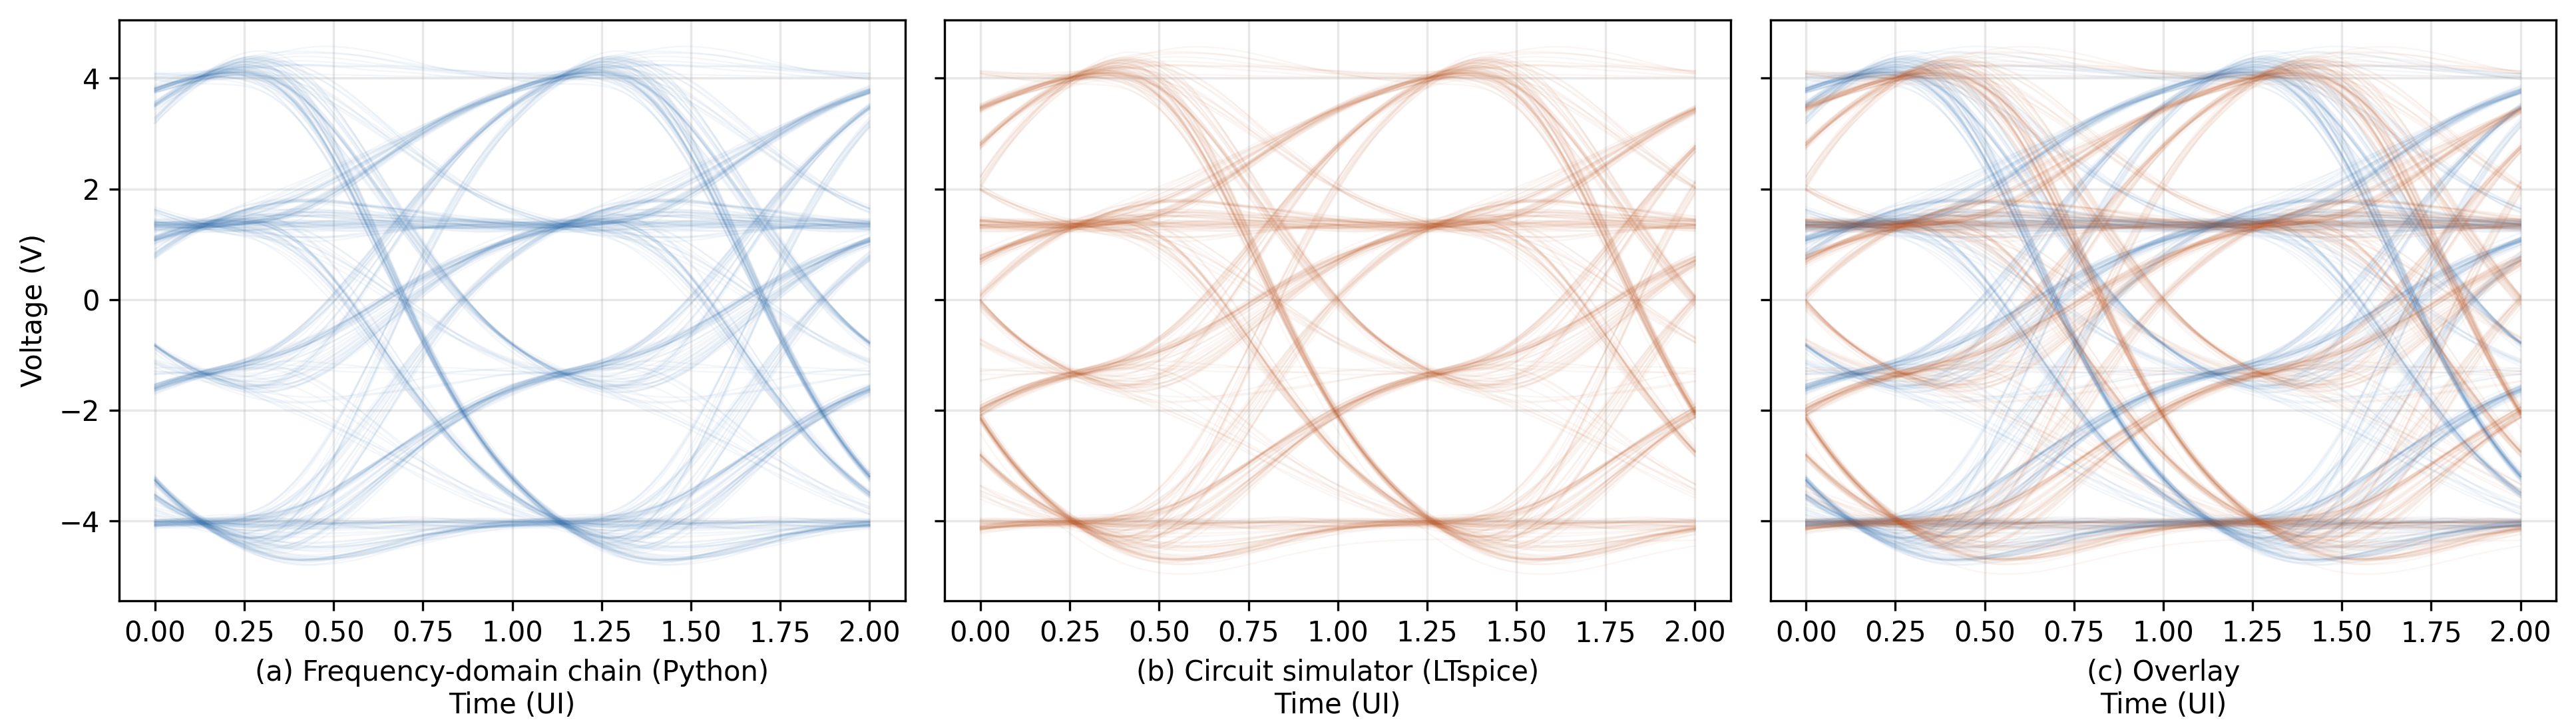
\includegraphics[width=\textwidth]{fig_ltspice_ojos.png}
\caption{PAM-4 eye diagram at 4~GBaud over the RC channel: (a)~chain
evaluated in the frequency domain, (b)~the same chain in a circuit
simulator (LTspice) excited with identical sequence and noise, and
(c)~overlay of both.}
\label{fig:ltspice}\end{figure*}

\subsection{Viable symbol rate per configuration and channel (rate reach)}
Table~\ref{tab:r1} reports the viable rate per channel and configuration
for the two criteria, and Fig.~\ref{fig:ratesweep} shows the BER sweeps.
At equal loss at Nyquist (\textit{equal\_il}), \emph{without equalization
the dispersive channels tolerate a higher rate than the RC} (4.6 and 5.2
versus 2.9~GBaud): the diffusive RC channel is the most pessimistic
because of its prolonged ISI tail. Under fixed physical length
(\textit{fixed}), the real 10-inch traces are very capable (FFE+CTLE+DFE
reaches 27.2~GBaud on FR-4 and exceeds 60~GBaud on Megtron~6 after
extending the sweep). On Megtron~6 \textit{fixed}, \emph{over-equalization}
is observed: FFE+CTLE reduces the viable rate (16.3 versus 40.1~GBaud
unequalized) because the CTLE amplifies noise unnecessarily over an almost
lossless channel.

\begin{table}[!t]
\caption{Viable symbol rate (GBaud, mean $\pm$ standard deviation, 30
realizations; $\mathrm{BER}\le10^{-2}$). EQ inherited from the RC.}
\label{tab:r1}\centering
\begin{tabular}{llccc}
\hline
\textbf{Crit.} & \textbf{Channel} & \textbf{No EQ} & \textbf{FFE+CTLE} & \textbf{+DFE} \\
\hline
\textit{eq\_il} & RC ($N{=}5$)   & $2.88{\pm}0.01$ & $9.76{\pm}0.18$ & $13.73{\pm}0.29$ \\
\textit{eq\_il} & FR-4 (22.9'')  & $4.58{\pm}0.11$ & $9.31{\pm}0.23$ & $9.71{\pm}0.23$ \\
\textit{eq\_il} & Megtron (36.9'')& $5.16{\pm}0.21$ & $10.83{\pm}0.28$ & $11.88{\pm}0.41$ \\
\hline
\textit{fixed}  & FR-4 (10'')    & $12.75{\pm}0.28$ & $14.06{\pm}0.31$ & $27.19{\pm}0.49$ \\
\textit{fixed}  & Megtron (10'') & $40.1{\pm}1.3$ & $16.27{\pm}0.15$ & $\ge 64^{\ast}$ \\
\hline
\end{tabular}
\par\smallskip
\footnotesize{$^{\ast}$ The sweep was extended to 64~GBaud to resolve the
saturations; the FFE+CTLE+DFE case on Megtron~6 still does not cross the
$10^{-2}$ threshold within the sweep and is reported as a lower bound (at a
$10^{-4}$ threshold the viable rate is finite, $\approx56$~GBaud;
Table~\ref{tab:rumbral}).}
\end{table}

\begin{figure*}[!t]\centering

\includegraphics[width=0.49\textwidth]{fig_barrido_tasa_equal_il.png}\hfill

\includegraphics[width=0.49\textwidth]{fig_barrido_tasa_fixed.png}
\caption{Semi-analytical BER versus PAM-4 symbol rate (median and envelope
over 30 realizations) for no equalization, FFE+CTLE and FFE+CTLE+DFE.
Left: equal-loss-at-Nyquist criterion; right: fixed physical length of
10~inches.}
\label{fig:ratesweep}\end{figure*}

\subsection{Signal integrity: eye diagram}
Fig.~\ref{fig:ojos} shows the PAM-4 eye diagrams at the operating point
(4~GBaud) over the physical channel: without equalization the eye is
closed, and the co-design chain progressively recovers it (FFE, FFE+CTLE)
until the DFE tightens the decision levels. Table~\ref{tab:r2} quantifies
the worst-eye opening per scenario and channel: it is negative without
equalization (closed eye) and positive at all equalized stages. The RC
channel reaches a larger opening after the CTLE than the dispersive
channels (a more modest opening despite the same boost), which anticipates
that the inherited co-design is not adapted to the physical channel
(Table~\ref{tab:r4}).

\begin{table}[!t]
\caption{Worst-eye opening (V) at the operating point (4~GBaud).}
\label{tab:r2}\centering
\begin{tabular}{lcccc}
\hline
\textbf{Channel} & \textbf{No EQ} & \textbf{FFE} & \textbf{FFE+CTLE} & \textbf{+DFE} \\
\hline
RC ($N{=}5$) & $-1.78$ & $+0.51$ & $+2.14$ & $+2.19$ \\
FR-4         & $-0.29$ & $+0.30$ & $+0.66$ & $+0.83$ \\
Megtron 6    & $-0.16$ & $+0.28$ & $+0.60$ & $+0.65$ \\
\hline
\end{tabular}
\end{table}

\begin{figure*}[!t]\centering
\includegraphics[width=\textwidth]{fig_ojo_escenarios.png}
\caption{PAM-4 eye diagrams at 4~GBaud (FR-4 channel): A (no
equalization), B (FFE), C (FFE+CTLE) and sampled levels with and without
DFE.}
\label{fig:ojos}\end{figure*}

\subsection{Reliability: BER at the operating point}
The reliability behavior is consistent with the viable rate
(Table~\ref{tab:r1}): at 4~GBaud, without equalization the RC channel is
not viable (BER $7.4\times10^{-2}$, above the threshold, since its limit
rate of 2.9~GBaud lies below the operating point), whereas the dispersive
channels are viable ($4.6\times10^{-3}$ and $2.4\times10^{-3}$). All
equalized configurations operate below the pre-FEC threshold
(Table~\ref{tab:r3}). Note that the equalized RC reaches $<10^{-12}$ while
the dispersive channels remain around $10^{-6}$: the equalization
inherited from the RC, although sufficient, is not adapted to the physical
channel, which motivates the re-co-design (Table~\ref{tab:r4}).

\begin{table}[!t]
\caption{Semi-analytical BER per scenario and channel (4~GBaud).}
\label{tab:r3}\centering
\begin{tabular}{lcccc}
\hline
\textbf{Channel} & \textbf{No EQ} & \textbf{FFE} & \textbf{FFE+CTLE} & \textbf{+DFE} \\
\hline
RC ($N{=}5$) & $7.4{\times}10^{-2}$ & $1.6{\times}10^{-10}$ & $<10^{-12}$ & $<10^{-12}$ \\
FR-4         & $4.6{\times}10^{-3}$ & $1.3{\times}10^{-6}$ & $4.9{\times}10^{-6}$ & $3.4{\times}10^{-7}$ \\
Megtron 6    & $2.4{\times}10^{-3}$ & $1.8{\times}10^{-6}$ & $4.5{\times}10^{-6}$ & $2.6{\times}10^{-6}$ \\
\hline
\end{tabular}
\end{table}

\subsection{BER-estimator validation and threshold sensitivity}
To rule out that the semi-analytical estimator overestimates performance,
it was contrasted against direct Monte Carlo counting over long sequences
($\approx5\times10^{5}$ symbols per point), using the same decision
thresholds (Fig.~\ref{fig:bermc}). In the region near the pre-FEC
threshold both estimates agree---for example, FR-4 with FFE+CTLE yields
$2.4\times10^{-2}$ (semi-analytical) versus $2.3\times10^{-2}$ (Monte
Carlo) at $16$~GBaud---; below the threshold the estimator is
\emph{slightly conservative} (it predicts more errors than the counting),
also with the decision feedback in the loop. Consequently, the reported
viable rates are not optimistic: the Gaussian assumption does not inflate
performance in the region that defines viability.

\begin{figure}[!t]\centering

\includegraphics[width=\linewidth]{fig_validacion_ber_mc.png}
\caption{Validation of the semi-analytical BER (lines) against Monte Carlo
counting (markers) for FR-4 and Megtron~6, FFE+CTLE and FFE+CTLE+DFE
scenarios.}
\label{fig:bermc}\end{figure}

The sequence length per realization ($1000$ symbols, $\approx250$ per
PAM-4 level) is sufficient because the semi-analytical estimator relies on
the per-level means and standard deviations---which converge with the
number of samples per level---and not on counting rare errors, and because
the viable rate is averaged over 30 realizations (effectively
$\sim\!7500$ symbols per level). A convergence study confirms this: when
increasing the length from $1000$ to $16000$ symbols, the viable rate
varies by less than $0.3\%$ (FR-4 FFE+CTLE $13.78\!\rightarrow\!13.74$;
FR-4 +DFE $27.12\!\rightarrow\!27.11$; Megtron~6 FFE+CTLE
$16.73\!\rightarrow\!16.77$~GBaud) and the per-level standard deviations
remain within $5\%$, so that the eye means and standard deviations are
converged at the operating point.

The definition of viability depends on the assumed pre-FEC threshold.
Table~\ref{tab:rumbral} reports the viable rate of the full chain at three
thresholds ($10^{-2}$, $10^{-3}$, $10^{-4}$): although the absolute value
decreases as a stricter threshold is required, the \emph{ordering} between
channels and the relative advantage of equalization are preserved, so that
the conclusions do not depend critically on the chosen threshold.

\begin{table}[!t]
\caption{FFE+CTLE+DFE viable rate (GBaud, mean $\pm$ standard deviation, 30
realizations) at different pre-FEC thresholds.}
\label{tab:rumbral}\centering
\begin{tabular}{llccc}
\hline
\textbf{Crit.} & \textbf{Channel} & $\mathbf{10^{-2}}$ & $\mathbf{10^{-3}}$ & $\mathbf{10^{-4}}$ \\
\hline
\textit{eq\_il} & RC ($N{=}5$)   & $13.7{\pm}0.3$ & $11.1{\pm}0.2$ & $9.8{\pm}0.1$ \\
\textit{eq\_il} & FR-4           & $9.7{\pm}0.2$  & $7.0{\pm}0.2$  & $5.7{\pm}0.2$ \\
\textit{eq\_il} & Megtron 6      & $11.9{\pm}0.5$ & $7.6{\pm}0.3$  & $5.8{\pm}0.3$ \\
\hline
\textit{fixed}  & FR-4           & $27.2{\pm}0.5$ & $19.0{\pm}0.8$ & $14.6{\pm}0.6$ \\
\textit{fixed}  & Megtron 6      & $\ge 64$       & $\ge 64$       & $56.4{\pm}1.7$ \\
\hline
\end{tabular}
\end{table}

\subsection{Transferability and re-co-design of the equalization}
The co-design optimized on the RC channel is not optimal for the physical
channel. Re-optimizing $(\omega_z, c_{post})$ per substrate (maximizing
the FFE+CTLE viable rate), the improvement is decisive on the realistic
channels: under \textit{fixed}, FR-4 goes from 14.1 to 24.2~GBaud
($+72\%$) and Megtron~6 from 16.3 to 32~GBaud ($+96\%$)
(Table~\ref{tab:r4}, Fig.~\ref{fig:redoe}). The optimal CTLE zero grows
with the channel bandwidth ($2.35\rightarrow2.65\rightarrow5.35\rightarrow
9.85$~GHz): short low-loss lines are wideband and require the boost at a
much higher frequency than the RC. As a caveat, the re-DoE maximizes
FFE+CTLE; in the presence of a DFE a softer CTLE is preferable (on FR-4
\textit{fixed}, the chain with DFE drops from 27.2 to 24.5~GBaud with the
aggressive EQ), which motivates a joint co-optimization of CTLE and DFE.

\begin{table}[!t]
\caption{Re-DoE: FFE+CTLE viable rate (GBaud) with EQ inherited from the RC
against EQ re-optimized per substrate.}
\label{tab:r4}\centering
\begin{tabular}{llccc}
\hline
\textbf{Crit.} & \textbf{Channel} & \textbf{$\omega_z$ re-opt} & \textbf{EQ-RC} & \textbf{re-opt.} \\
\hline
\textit{eq\_il} & FR-4 & $2.35$~GHz & $9.3{\pm}0.2$ & $9.6{\pm}0.2$ \\
\textit{eq\_il} & Megtron & $2.65$~GHz & $10.8{\pm}0.3$ & $11.9{\pm}0.6$ \\
\textit{fixed}  & FR-4 & $5.35$~GHz & $14.1{\pm}0.3$ & $24.2{\pm}0.4$ \\
\textit{fixed}  & Megtron & $9.85$~GHz & $16.3{\pm}0.2$ & $\ge 32^{\ast}$ \\
\hline
\end{tabular}
\par\smallskip
\footnotesize{$^{\ast}$ Saturates at the maximum of the sweep (32~GBaud);
lower bound. Mean $\pm$ standard deviation over 30 realizations.}
\end{table}

\begin{figure}[!t]\centering

\includegraphics[width=\linewidth]{fig_redoe_fixed.png}
\caption{Viable rate (\textit{fixed} criterion) with the equalization
inherited from the RC against the one re-optimized per substrate, for
FFE+CTLE and FFE+CTLE+DFE.}
\label{fig:redoe}\end{figure}

\subsection{Joint co-optimization of linear boost and feedback}
Optimizing the linear equalizer in isolation can degrade the full chain:
on a 10-inch FR-4 trace, the tuning that maximizes the linear eye opening
reduces the viable rate with decision feedback from $27.3$ to $25.1$~GBaud,
even below the inherited co-design. When jointly optimizing both stages,
taking the full chain as the objective, the linear equalizer is softer
(its zero drops from approximately $4.9$ to $1.6$~GHz) and the viable rate
rises to $28.2$~GBaud (Table~\ref{tab:r5}, Fig.~\ref{fig:coopt}); the
decision feedback cancels the tail interference that the linear boost no
longer needs to compensate \citep{11169790,11346689}. Quantitatively, the
staged optimization loses $8.1\%$ of rate relative to the inherited one,
whereas the joint one exceeds it; the improvement of the joint
co-optimization over the staged one reaches $\mathbf{12.4\%}$ on the
10-inch FR-4 trace (Table~\ref{tab:r5}). This difference constitutes the
main methodological contribution of the work: the linear boost and the
decision feedback must be co-optimized taking the full chain as the
objective, and not tuned in cascade, since maximizing the linear eye in
isolation can be counterproductive.

\begin{table}[!t]
\caption{Contribution of the joint co-optimization: viable rate of the
full chain with decision feedback (GBaud, mean $\pm$ standard deviation, 15
realizations) against the staged optimization. The isolated optimization
of the linear boost \emph{degrades} the chain; the joint one exceeds it.}
\label{tab:r5}\centering
\begin{tabular}{llcccc}
\hline
\textbf{Crit.} & \textbf{Channel} & \textbf{Inher.} & \textbf{Staged} & \textbf{Joint} & \textbf{$\Delta$ joint$-$staged} \\
\hline
\textit{eq\_il} & FR-4      & $9.7$ & $9.6$ & $9.9$ & $+0.3$ ($+3.1\%$) \\
\textit{eq\_il} & Megtron 6 & $11.8$ & $12.1$ & $12.1$ & $+0.0$ ($0\%$) \\
\textit{fixed}  & FR-4      & $27.3$ & $25.1$ & $28.2$ & $\mathbf{+3.1}$ ($\mathbf{+12.4\%}$) \\
\textit{fixed}  & Megtron 6 & $\ge 32^{\ast}$ & $\ge 32^{\ast}$ & $\ge 32^{\ast}$ & --- (sat) \\
\hline
\end{tabular}
\par\smallskip
\footnotesize{$^{\ast}$ Saturates at the maximum of the sweep (32~GBaud)
and does not discriminate between strategies. Typical standard deviations
$\le0.4$~GBaud.}
\end{table}

\begin{figure}[!t]\centering

\includegraphics[width=\linewidth]{fig_coopt_fixed.png}
\caption{Viable rate of the full chain with inherited equalization,
stage-optimized and jointly co-optimized (fixed-length criterion).}
\label{fig:coopt}\end{figure}

\subsection{Timing margin and robustness to jitter}
The horizontal margin was evaluated through the error-rate curve versus
the sampling phase. The horizontal opening reflects the same mismatch as
the vertical margin: the RC channel reaches $0.51$ of a unit interval
after the linear equalizer, against $0.18$ and $0.15$ on FR-4 and
Megtron~6 (Fig.~\ref{fig:banera}). With the feedback equalizer in the
loop, the two-dimensional margin follows the vertical one and the choice
of linear equalizer does not alter the horizontal margin, in line with the
voltage--timing margin trade-off described for high-speed links
\citep{4509472}. The injection of random and deterministic jitter
(Fig.~\ref{fig:estres}) shows that, in the considered test bench, the
viable rate does not degrade appreciably up to a deterministic jitter on
the order of $0.2$ to $0.25$ of a unit interval, and that the closure
level depends on the assumed model: close to $0.35$ with a dual-Dirac
worst-case representation, and to $0.4$ with sinusoidal periodic jitter
\citep{805809,7202856,10584882,7571656}.

\begin{figure}[!t]\centering

\includegraphics[width=\linewidth]{fig_banera_escenarios.png}
\caption{Error rate versus sampling phase (horizontal eye opening) per
equalization stage on the FR-4 channel.}
\label{fig:banera}\end{figure}

\begin{figure}[!t]\centering
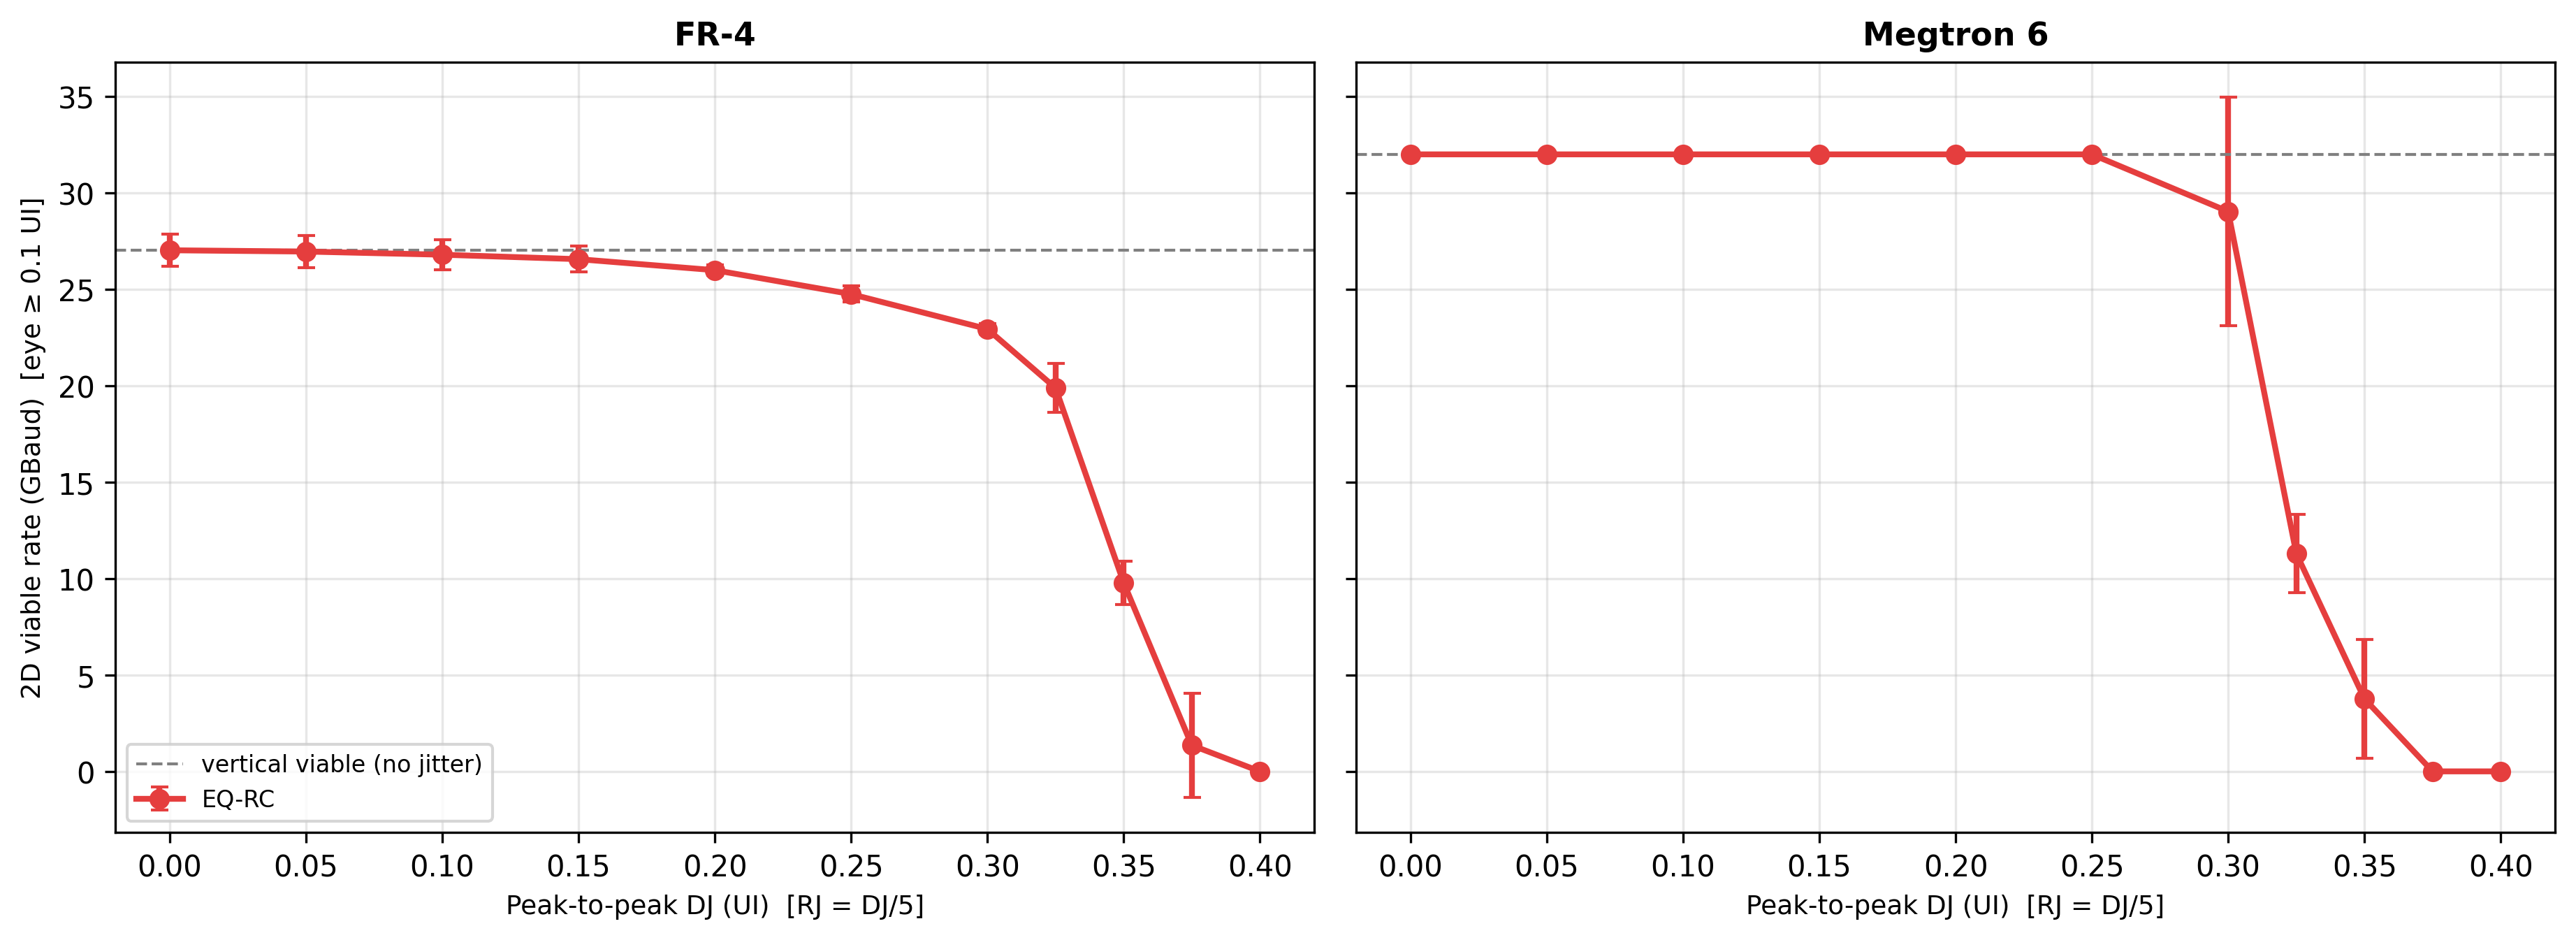
\includegraphics[width=\linewidth]{fig_estres_jitter.png}
\caption{Two-dimensional viable rate as a function of the injected
deterministic jitter, for the inherited and the co-optimized
equalization.}
\label{fig:estres}\end{figure}

\subsection{Generalization: PAM-8 with the same equalization chain}
Applying the co-design to PAM-8 (eight levels in $\pm3$~V) without
re-optimization, the order A $<$ B $<$ C in BER is preserved
(Fig.~\ref{fig:pam8ber}). The viable gross throughput of PAM-8 does not
exceed that of PAM-4: they coincide with FFE+CTLE and PAM-4 exceeds it
without equalization and with FFE+CTLE+DFE
(Tables~\ref{tab:r4a}--\ref{tab:r4b}, Fig.~\ref{fig:throughput}). The
rates in this comparison come from an independent PAM-4/PAM-8 sweep on a
$1\,\mathrm{GBaud}$ grid under identical channel and co-design, so the
PAM-4 values ($2,9,14$~GBaud) differ from Table~\ref{tab:r1}
($2.88,9.76,13.73$~GBaud) because of the sweep granularity (no
interpolation); the PAM-4 versus PAM-8 comparison is valid because both
share the same grid.

\begin{table}[!t]
\caption{Viable rate (GBaud, $\mathrm{BER}\le10^{-2}$; sweep on a 1~GBaud
grid, no interpolation).}
\label{tab:r4a}\centering
\begin{tabular}{lcc}
\hline
\textbf{Configuration} & \textbf{PAM-4} & \textbf{PAM-8} \\
\hline
No equalization & 2 & 1 \\
FFE + CTLE & 9 & 6 \\
FFE + CTLE + DFE & 14 & 8 \\
\hline
\end{tabular}
\end{table}

\begin{table}[!t]
\caption{Viable gross throughput (Gb/s) $=$ viable rate $\times$ bits per
symbol, without discounting FEC overhead.}
\label{tab:r4b}\centering
\begin{tabular}{lcc}
\hline
\textbf{Configuration} & \textbf{PAM-4} & \textbf{PAM-8} \\
\hline
No equalization & 4 & 3 \\
FFE + CTLE & 18 & 18 \\
FFE + CTLE + DFE & 28 & 24 \\
\hline
\end{tabular}
\end{table}

\begin{figure}[!t]\centering

\includegraphics[width=\linewidth]{fig_pam8_ber.png}
\caption{Semi-analytical BER versus symbol rate for PAM-8, in the three
equalization configurations.}
\label{fig:pam8ber}\end{figure}

\begin{figure}[!t]\centering

\includegraphics[width=\linewidth]{fig_throughput.png}
\caption{Viable gross throughput (Gb/s) per equalization configuration,
PAM-4 against PAM-8.}
\label{fig:throughput}\end{figure}

%% =====================================================================
\section{Discussion}
\label{sec:discussion}

The results support the hypothesis that equalization co-design maximizes
the viable symbol rate of the bandwidth-limited channel: the FFE+CTLE
linear equalization and the subsequent addition of the DFE successively
raise that rate above the intrinsic limit of the channel. The magnitude of
the increase depends on the adopted reference---the theoretical limit at
which the Nyquist frequency equals the bandwidth, or the viable rate
measured without equalization---so it is best interpreted as a
multiplicative factor rather than as a single figure. That the ladder
approximation reproduces the reference result supports the validity of the
simulator and confirms that the sweep measures the intended phenomenon and
not a numerical artifact.

The extension to dispersive physical channels qualifies the role of the RC
model. At equal insertion loss at the Nyquist frequency, the channels with
frequency-dependent losses tolerate, without equalization, a higher rate
than the RC channel, whose diffusive response presents a more prolonged
ISI tail \citep{8861405}; the RC model therefore tends to overestimate the
link difficulty at equal loss. Moreover, the co-design optimized on the RC
channel does not transfer without adjustment to the physical channel: the
optimal CTLE zero increases with the channel bandwidth, so re-optimizing
the equalization per substrate recovers viable rate, more appreciably on
short low-loss lines \citep{11169790}. This dependence is consistent with
the loss variation between laminates \citep{9785524,10385078,915226}. On
low-loss channels, linear equalization can even reduce the viable rate by
amplifying noise unnecessarily, which confirms that its usefulness is tied
to the channel severity.

The Megtron~6 fixed-length case deserves specific analysis for its
striking figures (without equalization, $40$~GBaud; with decision
feedback, above $60$). At $10$~inches, this low-loss-tangent laminate
($\tan\delta=0.004$) presents an insertion loss of barely $2$~dB at the
Nyquist frequency, so the channel hardly limits the signaling in the band
of interest: the factor that bounds performance is not the channel ISI but
the receiver---the input-referred noise and the finite bandwidth. In that
regime, the CTLE boost amplifies noise without appreciable ISI to
compensate, so linear equalization \emph{reduces} the viable rate
(over-equalization); the decision feedback, which cancels ISI without
amplifying noise, does not suffer that penalty and extends the rate up to
the limit imposed by the receiver noise. Far from being anomalous, this
behavior illustrates the central message of the work: the usefulness---and
even the sign---of each equalization stage's benefit depends on the
channel severity, so equalization must be sized on the specific physical
channel. It is worth noting that rates of several tens of GBaud in PAM-4
exceed the nominal operating point and must be interpreted as a limit of
the test bench---which does not incorporate reflections, vias or
crosstalk---and not as a deployment proposal.

The examination of the operating point qualifies this reading. At the
nominal rate, the transmit FFE alone already opens the eye, so there the
CTLE and DFE add margin, not viability; their value becomes apparent when
extending the rate, where the eye opening and the BER degrade abruptly.
This contrast warns that evaluating equalization at a single point can
misrepresent its role, and justifies adopting the rate reach as the
primary indicator. The addition of the DFE further illustrates that
equalization is not free: with the eye already open, the decision feedback
adds little and can slightly reduce the margin, consistent with the
erroneous-decision and error-propagation effects described for the DFE
\citep{10584882,9505189}. Its net benefit is therefore concentrated in the
severe-channel regime.

The PAM-8 stress case offers two observations. First, the performance
ordering between configurations is preserved when migrating to a denser
constellation, which indicates that the co-design---oriented to
compensating the channel and not the constellation---generalizes. Second,
under a fixed amplitude budget, the additional bits per symbol of PAM-8 do
not translate into higher viable gross throughput: its smaller reach
offsets the gain in bits and equals PAM-4 only with the full equalization
chain. This behavior is consistent with the margin penalty inherent to
higher modulation orders in bandwidth-limited systems \citep{8963973} and
with the motivation for PAM-4 as a compromise between spectral density and
robustness \citep{7964959}; it suggests that, on this channel, increasing
the baud rate dominates over increasing the modulation order.

Beyond the vertical amplitude margin, the horizontal timing margin was
examined by building the error-rate curve versus the sampling phase and
injecting random and deterministic jitter. With the decision-feedback
equalizer in the loop, the two-dimensional margin follows the vertical
one: in the considered test bench, the viable rate does not degrade
appreciably up to a deterministic jitter on the order of $0.2$ to $0.25$
of a unit interval, so for jitter budgets in that range the timing does
not limit the obtained reach \citep{7202856,10584882}. This voltage--timing
margin trade-off is consistent with the statistical margin simulation
frameworks for high-speed links \citep{4509472}. The jitter level that
closes the link depends on the assumed model---a dual-Dirac worst-case
representation places it near $0.35$ of a unit interval, while a sinusoidal
periodic jitter shifts it toward $0.4$ with a more gradual degradation
\citep{805809,7571656}---but in all cases the choice of linear equalizer
does not alter the horizontal margin, since the decision feedback cancels
the tail interference at each sampling instant.

The co-design of the linear and feedback stages deserves a clarification.
Optimizing the linear equalizer in isolation, maximizing the eye opening
before the feedback, can be counterproductive for the full chain: an
excessive boost opens the linear eye but amplifies noise that the feedback
stage would have avoided. Optimizing both stages jointly leads to a softer
linear equalizer that delegates the tail cancellation to the decision
feedback, in line with the convenience of co-designing the stages rather
than tuning them separately \citep{11169790,11346689}.

The scope of these results is bounded by several simplifications. The
dispersive line model incorporates skin effect and dielectric loss; the
surface roughness was treated through a first-order correction and a
sensitivity analysis bounded its effect (second order against dielectric
loss and length), but reflections from discontinuities and modal
dispersion are not modeled, and a rigorous validation would require
correlation with measured $S$-parameters or full-wave solvers
\citep{9134991,5089870}. As an intermediate step in that direction, the
chain was contrasted against an independent circuit simulator: it agrees in
the frequency response and, on the RC channel, in the time-domain eye
diagram, which indicates that the figures do not depend on the particular
implementation; the time-domain representation of the dispersive channel in
that simulator is limited by the non-rational nature of the skin-effect
loss, so its eye is evaluated in the frequency domain. The DFE is fitted
with the transmitted sequence, so its figures represent a performance bound
rather than a blind adaptive implementation. The ladder approximation
reproduces the RC line with a finite order, somewhat conservative in the
band that equalization exploits relative to the analytical transfer
function. The BER is a semi-analytical estimate under a Gaussian
assumption, suitable for avoiding the cost of Monte Carlo counting of low
error rates \citep{6248821}; it was validated against direct counting in the
region near the pre-FEC threshold, where both agree and the estimator is
slightly conservative, although it does not replace a characterization of
non-Gaussian tails at very low error rates; in that sense it is consistent
with the statistical-eye methods in the literature \citep{7202856,10415105}.
Finally, the co-design was explored in a two-variable subspace through
Latin hypercube sampling, amenable to extension with sequential or
Bayesian-optimization schemes \citep{11309336}, and the eye was evaluated at
a single operating point.

%% =====================================================================
\section{Conclusions}
\label{sec:conclusion}

The ladder approximation reproduces the analytical transfer function of the
RC channel and, on it, the reference result, which validates the
simulator. A cross-check in an independent circuit simulator, which
reproduces the frequency response of the chain and its eye diagram over the
RC channel, reinforces this validation. Replacing the RC model with a
transmission line with frequency-dependent losses confirms that the
physical channel is dispersive: its attenuation grows with frequency and
its magnitude depends on the substrate, with a propagation delay absent
from the diffusive model.

The equalization co-design raises the viable symbol rate above the limit of
the unequalized channel: linear equalization opens the eye diagram and the
decision-feedback equalizer extends the rate in the severe regime. The
comparison between channels qualifies this reading: at equal loss at the
Nyquist frequency, the dispersive channels tolerate a higher rate without
equalization than the RC channel, so the latter tends to overestimate the
link difficulty; under fixed physical length, by contrast, real traces are
considerably more capable.

The co-design optimized on the RC channel does not transfer without
adjustment to the physical channel. The optimal zero of the linear
equalizer increases with the channel bandwidth, so re-optimizing the
equalization per substrate recovers viable rate, more appreciably on short
low-loss lines. On those benign channels, a linear equalization that is too
aggressive can even reduce the viable rate by amplifying noise; jointly
co-optimizing the linear boost and the decision feedback, taking the full
chain as the objective, avoids this penalty and leads to a softer boost
that delegates the tail cancellation to the feedback.

The timing margin, evaluated with the error-rate curve versus the sampling
phase under random and deterministic jitter, is robust: with the decision
feedback in the loop, the horizontal margin follows the vertical one and,
in the considered test bench, does not degrade appreciably for
deterministic jitter up to the order of one fifth of a unit interval, so
the timing does not limit the obtained reach in that range.

The co-design generalizes to a denser constellation---the performance
ordering between configurations is preserved with eight-level
modulation---but under a fixed amplitude budget the higher modulation order
does not increase the viable gross throughput relative to four-level
modulation.

Equalization co-design maximizes the viable symbol rate of
bandwidth-limited interconnect channels, both on the validated RC model and
on dispersive physical channels; this gain is attributable to the
equalization---and not to optimistic receiver assumptions---since it was
evaluated with input-referred noise and finite bandwidth. The study further
shows that the co-design must be carried out on the physical channel and
not on its idealization.

As recommendations and future lines, it is suggested to refine the jitter
model toward more realistic distributions, to validate the dispersive model
against measured scattering parameters or full-wave solvers, to adopt
standard channel-operating-margin and statistical error-rate-estimation
metrics, and to validate the link experimentally on a physical trace with
hardware error counting.

%% =====================================================================
%% ===== Author statements required by the AEU/IJEC Guide for Authors =====

\section*{CRediT authorship contribution statement}
%% TO BE CONFIRMED by the authors. Proposed distribution; edit as needed.
\textbf{Segundo Francisco Segura-Altamirano:} Conceptualization,
Methodology, Software, Validation, Formal analysis, Investigation, Data
curation, Writing -- original draft, Visualization.
\textbf{Diana Mercedes Castro-C\'ardenas:} Conceptualization, Validation,
Resources, Supervision, Project administration, Writing -- review and
editing.

\section*{Declaration of competing interest}
The authors declare that they have no known competing financial interests
or personal relationships that could have appeared to influence the work
reported in this paper.

\section*{Funding}
This research did not receive any specific grant from funding agencies in
the public, commercial, or not-for-profit sectors.

\section*{Data availability}
%% AEU/IJEC follows Option C: deposit data in a repository and cite/link it,
%% or state why it cannot be shared. RECOMMENDED: deposit the simulation code
%% and result datasets in a repository (e.g. Zenodo or Mendeley Data), obtain a
%% DOI, and replace the sentence below with a citation/link to that dataset.
The simulation code and the datasets generated and analyzed in this study
are available from the corresponding author upon reasonable request.

%% \section*{Acknowledgements}  %% optional (TO BE COMPLETED, if applicable)

\section*{Declaration of generative AI and AI-assisted technologies in the manuscript preparation process}
During the preparation of this work, the authors used Claude Code and
Antigravity CLI in order to organize information, assist with data
analysis, structure the repository, and improve the drafting of the
manuscript. After using these tools, the authors reviewed and edited the
content as needed and take full responsibility for the content and results
of the published article.

%% Bibliography (Elsevier numbered / Vancouver style, required by AEU/IJEC)
\bibliographystyle{elsarticle-num}
\bibliography{references}

\end{document}
